% Parte 3: Open RAN

\section{O Conceito de Open RAN}

\begin{frame}{Diferenças: Open RAN, O-RAN e OpenRAN}
% \small
\begin{itemize}
  \item \textbf{Open RAN (conceito genérico)}  
    \begin{itemize}
      \item Termo amplo que se refere à \textbf{abertura e desagregação} das redes de acesso de rádio (RAN).  
      \item Não está ligado a um grupo ou organização específica.  
      \item Objetivo: evitar o \textit{vendor lock-in} e permitir múltiplos fornecedores.
    \end{itemize}

  \item \textbf{O-RAN (O-RAN Alliance)}  
    \begin{itemize}
      \item Iniciativa formal liderada por operadoras globais (ex.: AT\&T, China Mobile, NTT Docomo, etc.).  
      \item Define \textbf{especificações técnicas abertas}, interfaces e padrões de interoperabilidade.  
      \item Produz documentos, white papers e código aberto (ex.: \textit{O-RAN Software Community}).
    \end{itemize}

  \item \textbf{OpenRAN (Telecom Infra Project - TIP)}  
    \begin{itemize}
      \item Focado em \textbf{implementações práticas} (\textit{use cases}) de RAN aberta.  
      \item Visa acelerar \textbf{testes, protótipos e implantações comerciais}.  
      \item Complementa as especificações da O-RAN Alliance com atividades de campo.
    \end{itemize}
\end{itemize}
\end{frame}

\begin{frame}{Conceito de Open RAN}
\begin{itemize}
  \item Arquitetura aberta para redes de acesso rádio (RAN)
  \item Desagregação de componentes: RU, DU e CU
  \item Interfaces abertas e padronizadas (ex.: O-RAN Alliance)
  \item Interoperabilidade entre múltiplos fornecedores
  \item Uso de virtualização e servidores COTS
  \item Maior flexibilidade, inovação e redução de custos
\end{itemize}
\vspace{-0.2cm}
\begin{figure}
    \centering
    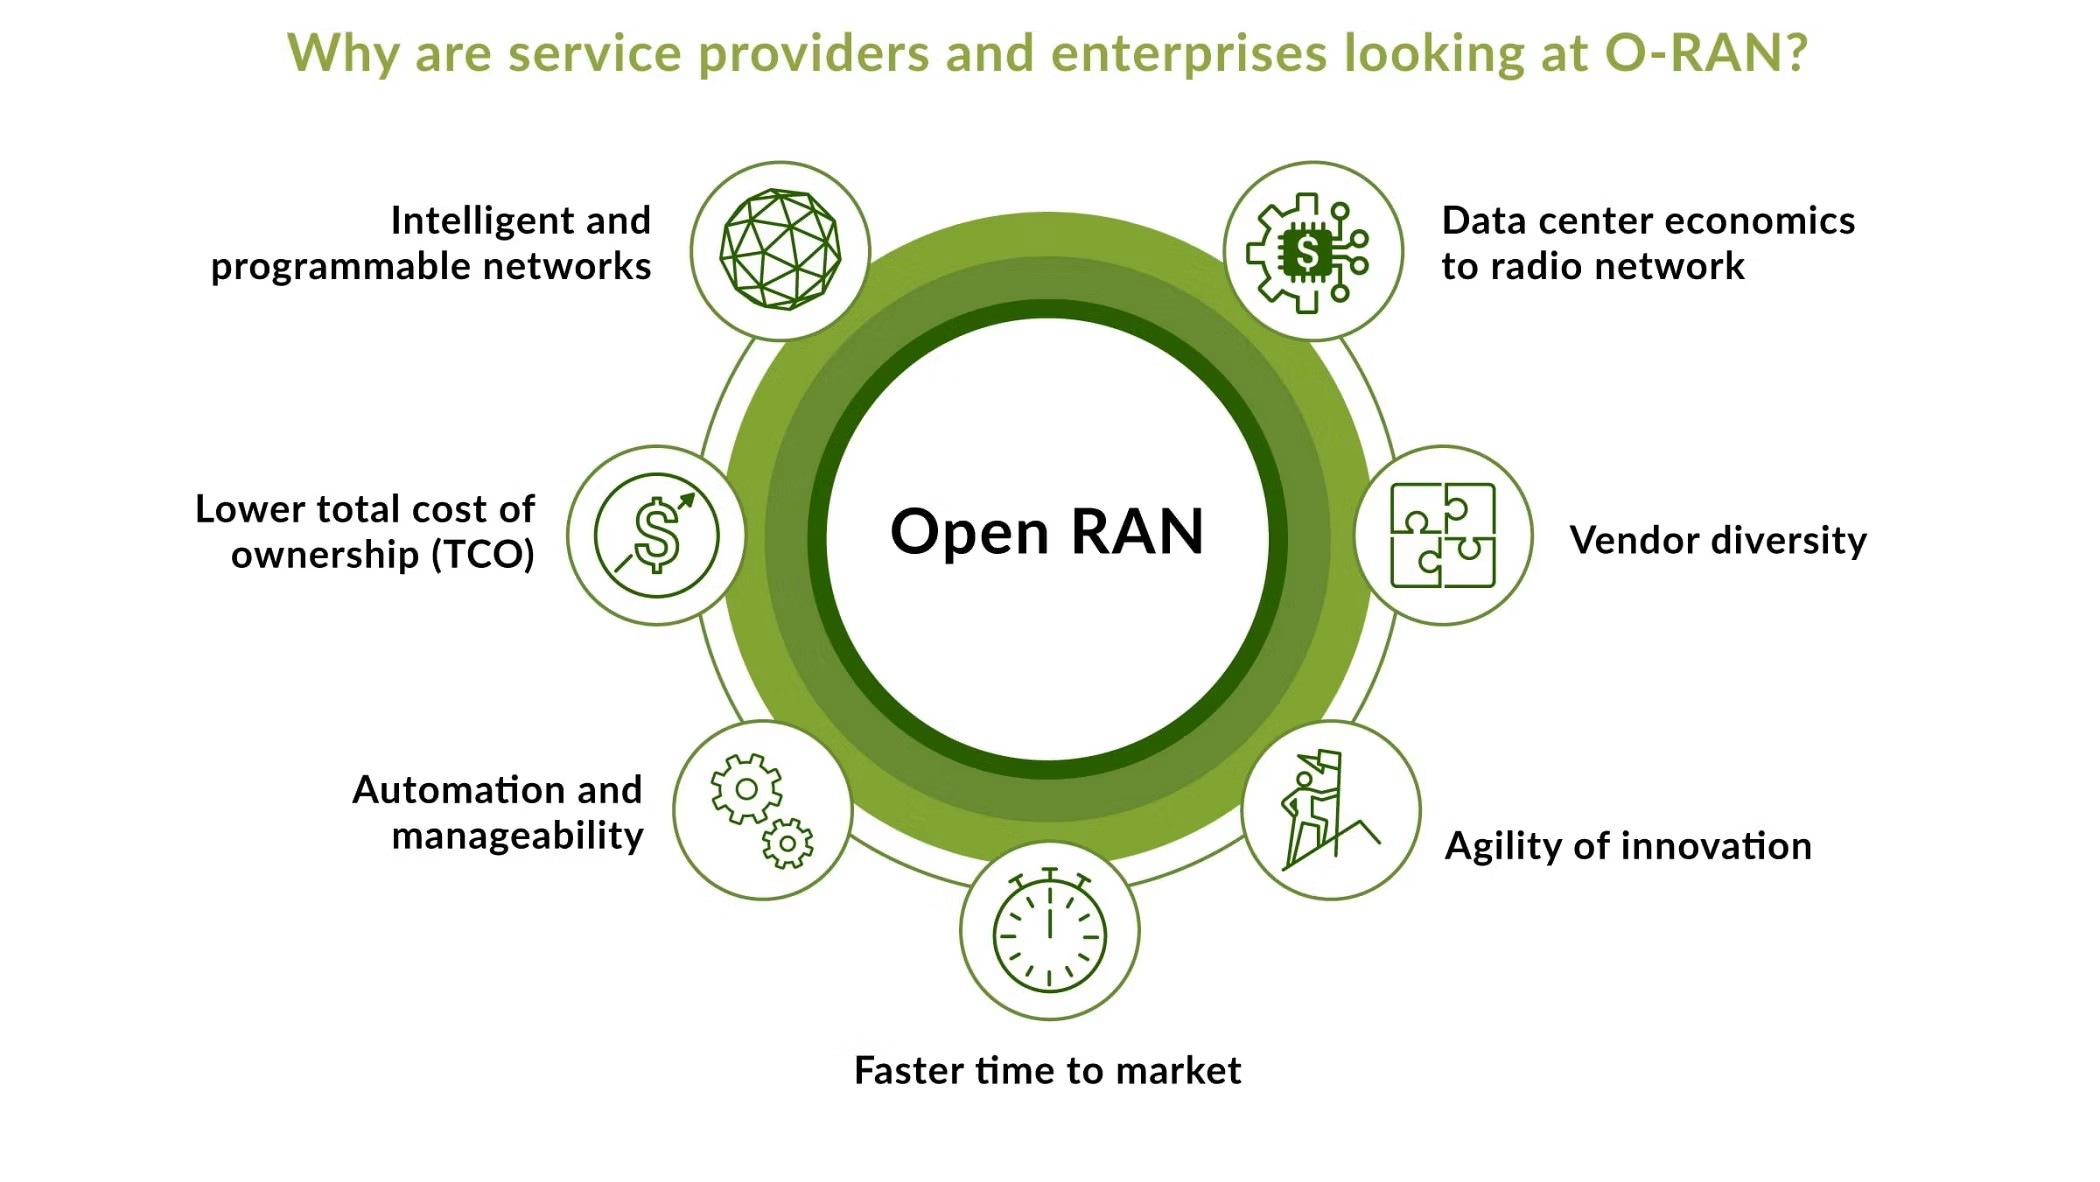
\includegraphics[width=0.6\linewidth]{figs/what-is-O-RAN.jpeg}
    \caption{O que \textit{stakeholders} procuram?\footnote{\href{https://www.juniper.net/us/en/research-topics/what-is-open-ran.html}{https://www.juniper.net/us/en/research-topics/what-is-open-ran.html}}}
\end{figure}
\end{frame}

\begin{frame}{Evolução até Open RAN}
\begin{figure}
    \centering
    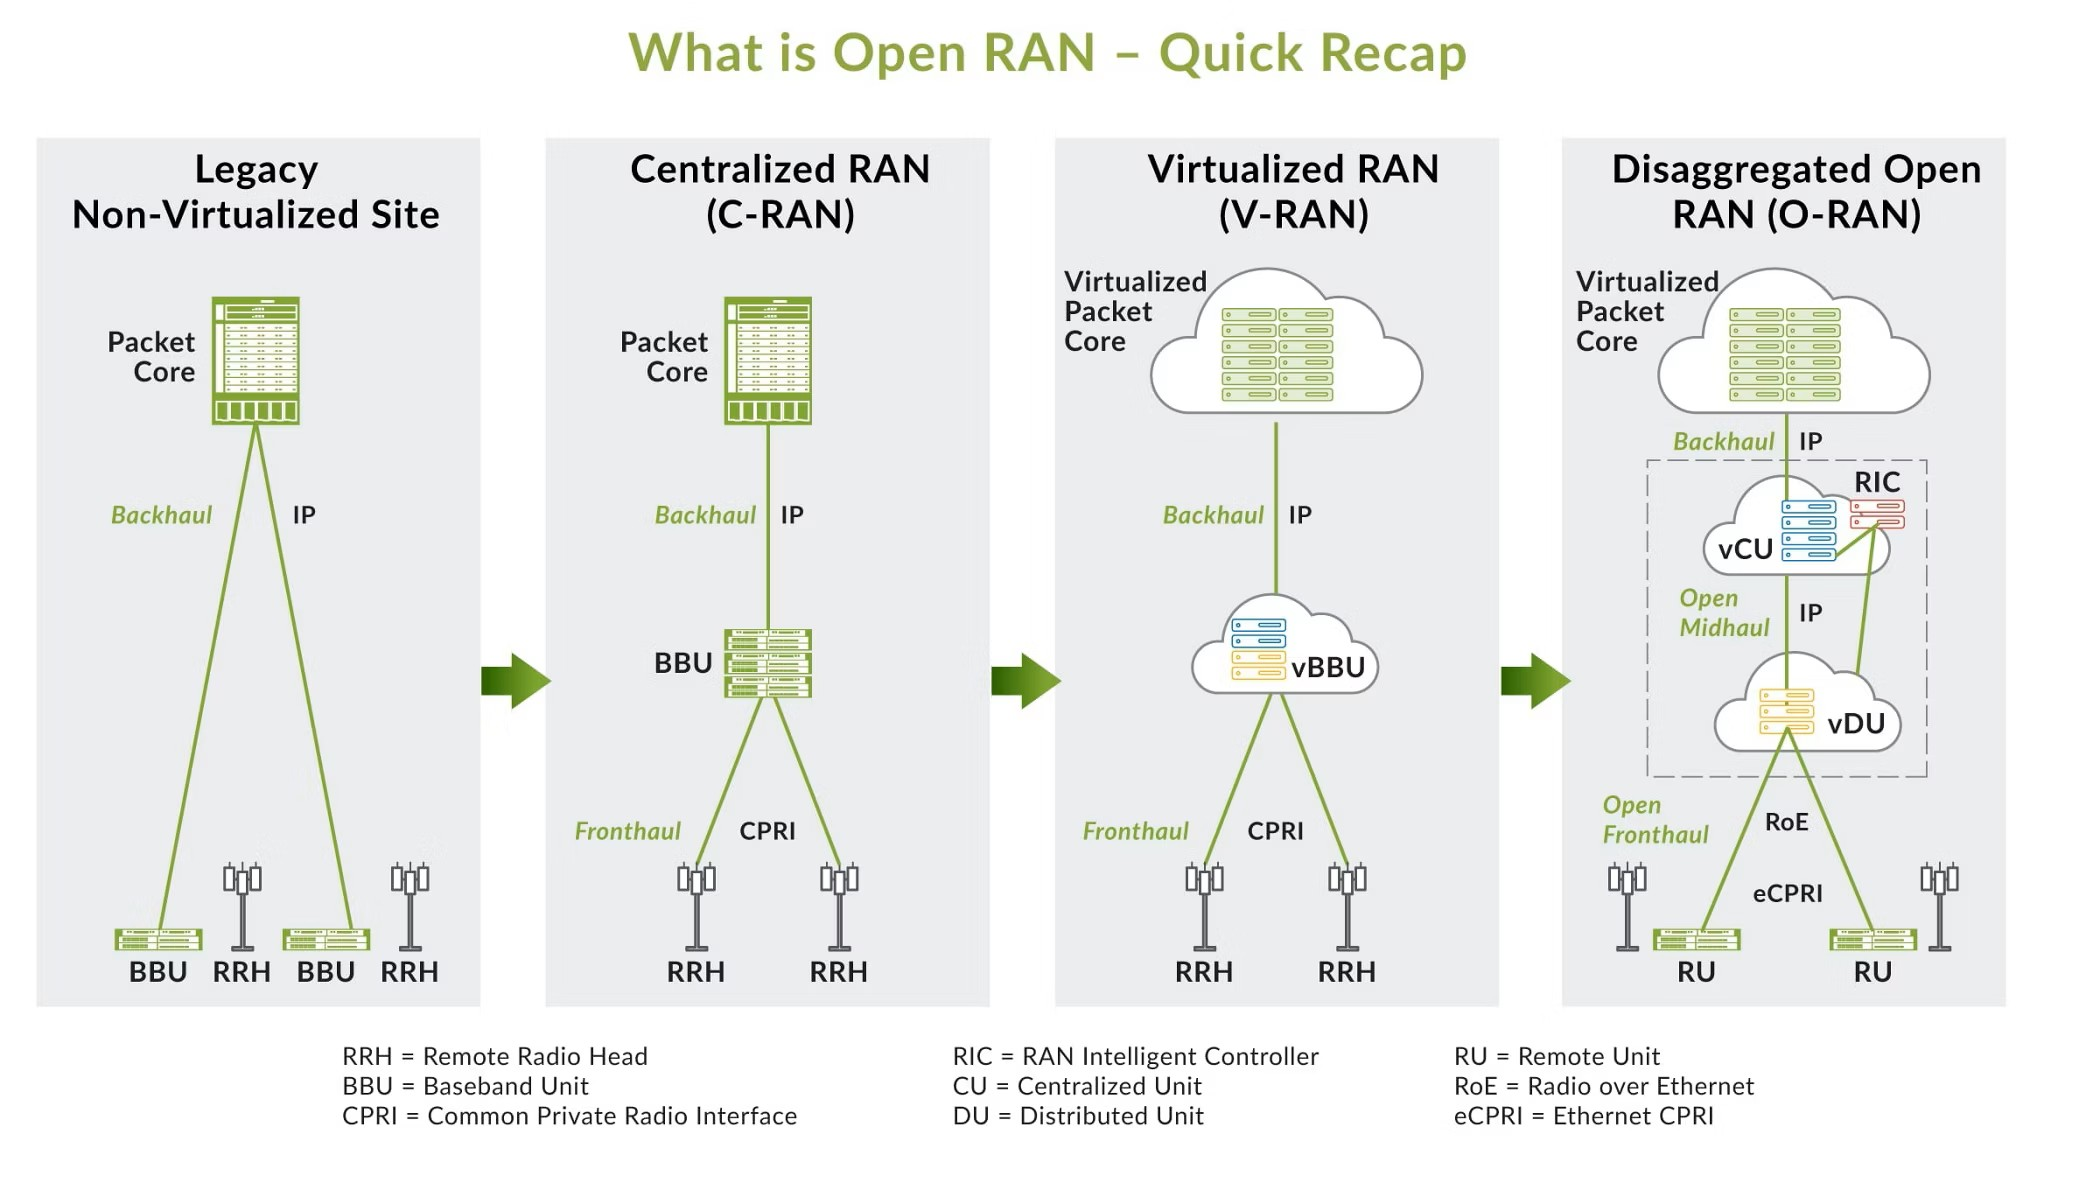
\includegraphics[width=\linewidth]{figs/what-is-O-RAN-quick-recap.jpeg}
    \caption{Recapitulando\footnote{\href{https://www.juniper.net/us/en/research-topics/what-is-open-ran.html}{https://www.juniper.net/us/en/research-topics/what-is-open-ran.html}}}
\end{figure}
\end{frame}

\begin{frame}{Arquitetura Open RAN\footcite{marques2023desagregando}}
\begin{columns}
    \begin{column}{0.5\textwidth}
    \begin{itemize}
      \item \scriptsize \textbf{SMO}: Gerenciamento e orquestração de toda a rede
    
      \item \textbf{Non-RT RIC}: Controle inteligente não em tempo real (políticas, ML/AI)
    
      \item \textbf{Near-RT RIC}: Controle quase em tempo real (10ms – 1s), otimizações dinâmicas
    
      \item \scriptsize \textbf{O-CU (Central Unit)}
            \begin{itemize}
              \item \scriptsize \textbf{O-CU-CP (Control Plane)}: sinalização e controle  
              \item \scriptsize \textbf{O-CU-UP (User Plane)}: encaminhamento de dados do usuário  
            \end{itemize}
    
      \item \scriptsize \textbf{O-DU (Distributed Unit)}: Processamento de tempo crítico (MAC, RLC, parte do PHY)  

      \item \scriptsize \textbf{O-RU (Radio Unit)}:  Processamento de rádio e funções da camada física (RF, mod/demod)  

    \end{itemize}
    \end{column}
    \begin{column}{0.5\textwidth}
        \vspace{0.5cm}
        \begin{figure}
            \centering
            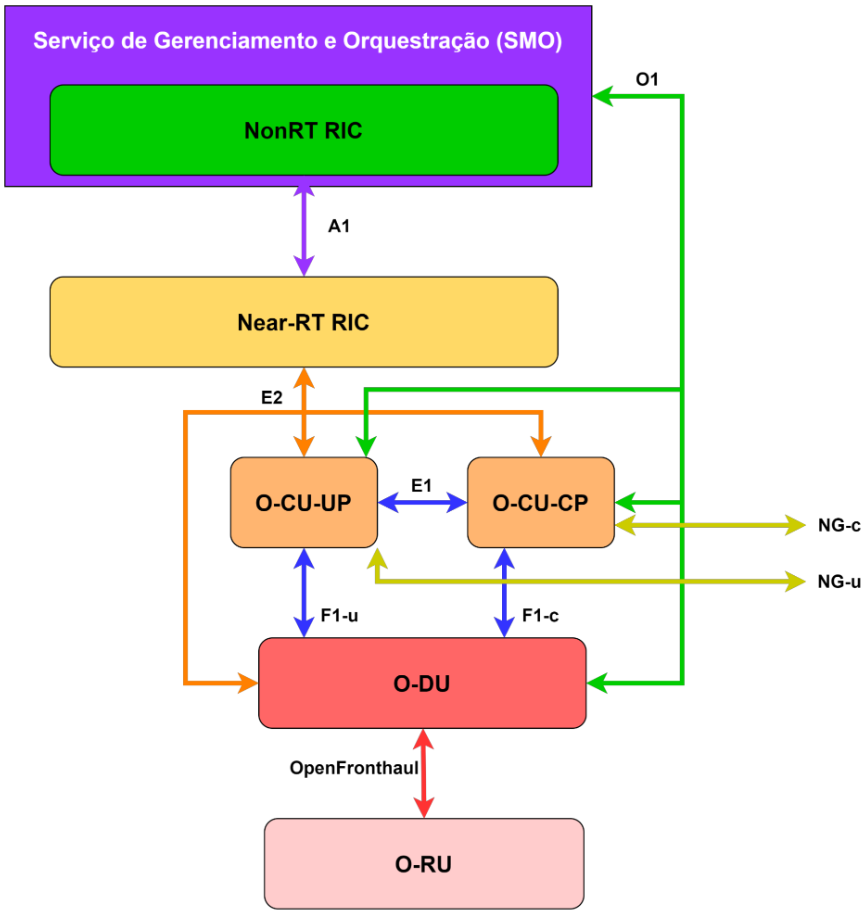
\includegraphics[width=\linewidth]{figs/arquitetura-openran.png}
            \caption{Arquitetura Open RAN\textsuperscript{4}}
        \end{figure}
    \end{column}
\end{columns}
\end{frame}

\begin{frame}{Benefícios do Open RAN}
\small
\begin{itemize}
  \item \textbf{Redução de custos CAPEX/OPEX}: uso de COTS e interfaces abertas diminui dependência de fornecedores proprietários, isso reduz investimentos iniciais e custos operacionais.
  \item \textbf{Flexibilidade e inovação}: arquitetura desagregada permite atualização modular e rápida integração de novas funcionalidades, estimulando experimentação tecnológica.
  \item \textbf{Novos players no mercado}: abertura do ecossistema cria oportunidades para startups, universidades e empresas de software, ampliando a competitividade e acelerando a evolução da rede.
  \item \textbf{Ecossistema colaborativo}: estímulo à padronização e à cooperação entre diferentes organizações, com maior diversidade de soluções e modelos de negócios.
\end{itemize}
\end{frame}

\begin{frame}{Desafios do Open RAN}
\small
\begin{itemize}
  \item \textbf{Interoperabilidade real}: necessidade de compatibilidade entre equipamentos e softwares de múltiplos fornecedores, exigindo testes extensivos e certificações.
  \item \textbf{Performance em cenários críticos}: manter níveis de latência, throughput e confiabilidade equivalentes às soluções proprietárias em ambientes de alta demanda (ex.: redes 5G industriais).
  \item \textbf{Segurança e confiabilidade}: abertura das interfaces amplia a superfície de ataque, demandando mecanismos robustos de autenticação, criptografia e monitoramento contínuo.
  \item \textbf{Resistência dos fornecedores tradicionais}: barreiras comerciais e estratégicas impostas por fabricantes estabelecidos que ainda dominam grande parte do mercado.
  \item \textbf{Complexidade de integração}: coordenação de múltiplos componentes heterogêneos aumenta os desafios de gerenciamento, operação e manutenção da rede.
\end{itemize}
\end{frame}